\documentclass[11pt ,a4paper , twoside , openright ]{article}
\usepackage[T1]{fontenc}
\usepackage[utf8]{inputenc}
\usepackage{lmodern}
\usepackage{hyperref}
\usepackage[a4paper,top=3cm,bottom=3cm,left=2.5cm,right=2.5cm]{geometry}
\usepackage[square,numbers]{natbib}
\bibliographystyle{abbrvnat}
\usepackage[italian]{babel}
\usepackage[usenames]{color} 
\usepackage{listings} 
\usepackage{color}
\usepackage{graphicx}
\usepackage[bottom]{footmisc}
\graphicspath{ {./images/} }
\definecolor{mygreen}{rgb}{0,0.6,0}
\definecolor{mygray}{rgb}{0.5,0.5,0.5}
\definecolor{mymauve}{rgb}{0.58,0,0.82}

\lstset{ 
	backgroundcolor=\color{white}, 
	basicstyle=\footnotesize,
	breakatwhitespace=false, 
	breaklines=true,
	captionpos=b, 
	commentstyle=\color{mygreen}, 
	escapeinside={\%*}{*)}, 
	extendedchars=true, 
	frame=single,
	keepspaces=true, 
	keywordstyle=\color{blue},
	morekeywords={*,...}, 
	numbers=left, 
	numbersep=5pt, 
	numberstyle=\tiny\color{mygray}, 
	rulecolor=\color{black}, 
	showspaces=false, 
	showstringspaces=false, 
	showtabs=false, 
	stepnumber=1, 
	stringstyle=\color{mymauve}, 
	tabsize=2, 
}

\definecolor{darkgray}{rgb}{.4,.4,.4}
\definecolor{purple}{rgb}{0.65, 0.12, 0.82}

\lstdefinelanguage{JavaScript}{
	keywords={typeof, new, true, false, catch, function, return, null, catch, switch, var, if, in, while, do, else, case, break},
	keywordstyle=\color{blue}\bfseries,
	ndkeywords={class, export, boolean, throw, implements, import, this},
	ndkeywordstyle=\color{darkgray}\bfseries,
	identifierstyle=\color{black},
	sensitive=false,
	comment=[l]{//},
	morecomment=[s]{/*}{*/},
	commentstyle=\color{purple}\ttfamily,
	stringstyle=\color{red}\ttfamily,
	morestring=[b]',
	morestring=[b]"
}

\lstset{
	language=JavaScript,
	extendedchars=true,
	basicstyle=\small\ttfamily,
	showstringspaces=false,
	showspaces=false,
	numbers=left,
	numberstyle=\scriptsize,
	numbersep=9pt,
	tabsize=2,
	breaklines=true,
	showtabs=false,
	captionpos=b
}

\author{
	Daniele Rigon - 857319 \\
}


\begin{document}
	
\title{Tesi - Geolocation API}
\maketitle
\pagebreak
\tableofcontents

\newpage
\section{Overview}
La Geolocation API viene utilizzata per ottenere la posizione geografica di un utente. 
Poiché questo può compromettere la privacy la posizione non è disponibile a meno che l'utente non la approvi: su un dispositivo mobile avremo un set di coordinate provenienti dal sensore GPS mentre su un portatile potremo usare il posizionamento legato all’ip della connessione internet.
\newpage
\section{Specifiche}

\subsection{Oggetto della geolocalizzazione}
Le API di geolocalizzazione sono pubblicate tramite l'oggetto navigator.geolocation. Se l'oggetto esiste, il servizio di geolocalizzazione è disponibile. Per testare l'esistenza di tale oggetto:
\lstinputlisting{code/GeolocationInNavigator.js}

\subsection{Metodi}
Ci sono solamente tre metodi a disposizione: getCurrentPosition, watchPosition e clearWatch. I primi due sono utili a ottenere la posizione corrente mentre il terzo serve ad annullare la ricerca della posizione corrente. 
La differenza tra i primi due va ricercata nella loro periodicità, mentre il primo metodo fornisce il dato una sola volta, il secondo si attiva automaticamente ogni qualvolta la posizione cambi, o ogni tot intervallo di tempo.
La sintassi per invocare questi metodi è la seguente:
\lstinputlisting{code/Sintassi.js}

\subsubsection{GetCurrentPosition}
\lstinputlisting{code/GetCurrentPosition.js}
L'esempio chiama la funzione dosomething() quando la posizione viene calcolata. \\
Un esempio concreto potrebbe essere il seguente\footnote{viene chiesto il permesso all'utente nell'uso della posizione quando si chiama il metodo GetCurrentPosition e WatchPosition; se negata apparirà un messaggio di errore in console, se consentita verranno mostrati i dati dell'utente}: \\
\pagebreak
\lstinputlisting{code/EsempioCompleto.js}
Che produrrà la seguente pagina:
\begin{figure}[h]
	\centering
	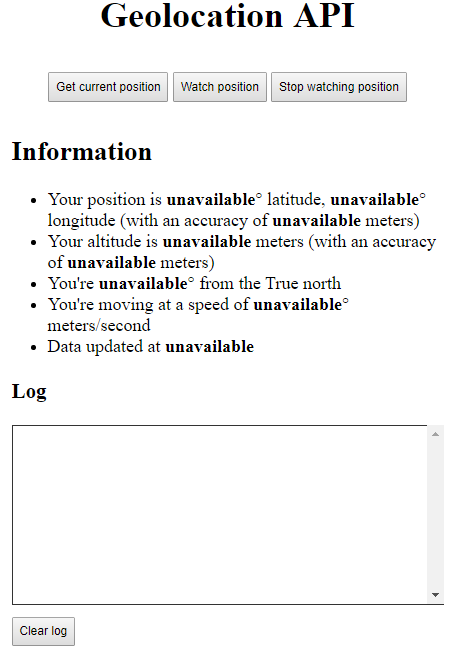
\includegraphics[width=0.5\linewidth]{geo1}
	\caption{Pagina info Geolocation}
	\label{fig: Pagina info Geolocation}
\end{figure}
\pagebreak
\\
Quando saranno chiamati i metodi getCurrentposition o WatchPosition verrà chiesto all'utente il permesso per usare la posizione.
\begin{figure}[h]
	\centering
	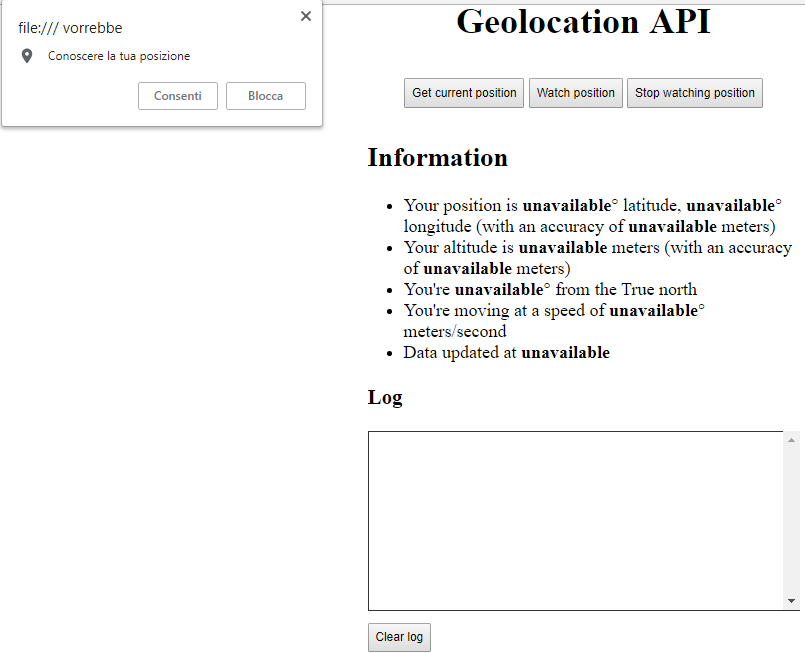
\includegraphics[width=0.4\linewidth]{geo2}
	\caption{Richiesta permesso}
	\label{fig: Richiesta permesso}
\end{figure}
\\
Se l'utente rifiuta la posizione non viene calcolata e viene mostrato un messaggio di errore in console.
\begin{figure}[h]
	\centering
	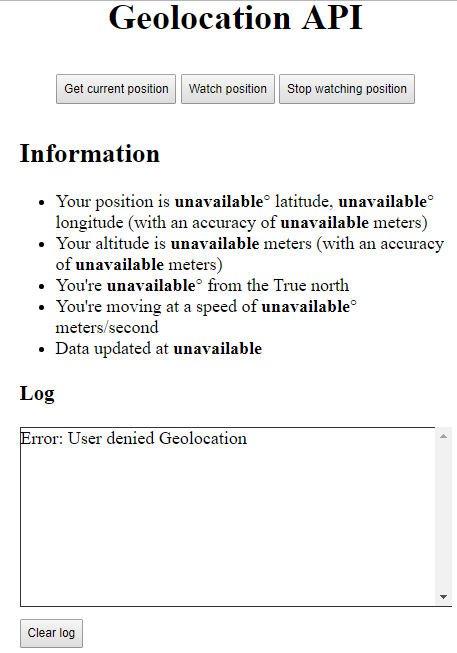
\includegraphics[width=0.4\linewidth]{geo3}
	\caption{Rifiuto autorizzazione}
	\label{fig: Rifiuto autorizzazione}
\end{figure}
\pagebreak
\\
Se l'utente acconsente all'utilizzo della posizione verrà mostrato un messaggio di conferma in console e saranno mostrate a video tutte le informazioni disponibili dell'utente.
\begin{figure}[h]
	\centering
	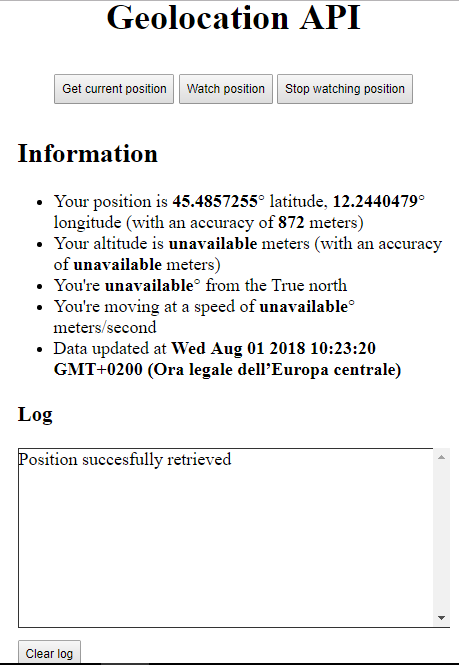
\includegraphics[width=0.5\linewidth]{geo4}
	\caption{Accetto autorizzazione}
	\label{fig: Accetto autorizzazione}
\end{figure}
\pagebreak
\subsubsection{WatchPosition}
Se la posizione cambia (perché il dispositivo si sposta o perché viene calcolata una posizione più accurata), si può settare una funzione che viene chiamata quando la posizione attuale si aggiorna. Basta usare la funzione watchPosition(), che ha gli stessi parametri di input di getCurrentPosition(). Questa funzione viene chiamata più volte così da permettere al browser di sapere sempre la posizione del dispositivo. La funzione di errore è opzionale come lo era per getCurrentPosition().
\lstinputlisting{code/WatchPosition.js}
Il metodo watchPosition() ritorna un ID numerico che può essere usato per identificare univocamente il controllo della posizione. 

\subsubsection{ClearPosition}
Viene usato il metodo clearWatch() per annullare il monitoraggio della posizione.
\lstinputlisting{code/ClearPosition.js}
\newpage
\section{Problemi sicurezza/privacy}
Uno dei principali problemi con la Geolocation API è rappresentato dagli attacchi di cross-site scripting (XSS) dovuto al fatto che gli oggetti per tracciare le coordinate (latitudine e longitudine) risiedono all'interno del DOM, il quale è accessibile con JavaScript e attraverso il quale potrebbe essere rubata la posizione dell'utente. 
Dato che gli utenti si fidano del sito web, si fidano anche della richiesta di posizione e la condividono.
Un problem importante è che se l'utente non disabilita il tracciamento il browser continuerà a esporre la posizione dell'utente all'attaccante.
\begin{figure}[h]
	\centering
	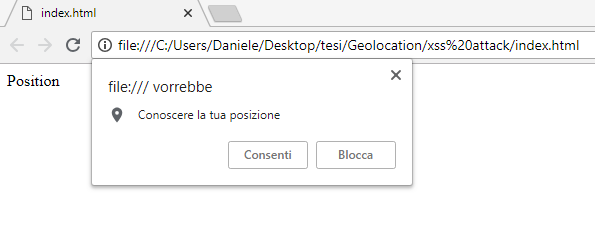
\includegraphics[width=1\linewidth]{pos1}
	\caption{Richiesta posizione}
	\label{fig: Richiesta posizione}
\end{figure}
\\
Supponiamo che un utente malintenzionato abbia rilevato una vulnerabilità XSS in un sito Web; tutto ciò che dovra fare è fare in modo che la vittima esegua il seguente codice JavaScript per rubare la posizione.
\lstinputlisting{code/script.js}
Il codice utilizza le proprietà del DOM cords.latitude e cords.langitude per determinare rispettivamente la latitudine / longitudine e le memorizza in una variabile. Successivamente il codice JavaScript invia i dati al dominio dell'attaccante, in modo diverso a seconda di come è stato configurata la richiesta.
\pagebreak
\\
Se l'utente non consente all'utilizzo della posizione non succederà nulla nella pagina.
\begin{figure}[h]
	\centering
	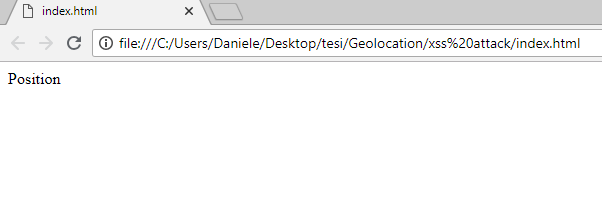
\includegraphics[width=1\linewidth]{Blocca}
	\caption{Blocca autorizzazione}
	\label{fig: Blocca autorizzazione}
\end{figure}
\\
Se l'utente acconsente all'utilizzo della posizione essa sarà calcolata e, risiedendo nel DOM, può esser facilmente rubata.
\begin{figure}[h]
	\centering
	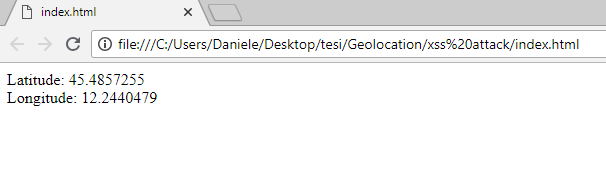
\includegraphics[width=1\linewidth]{Consenti}
	\caption{Consenti autorizzazione}
	\label{fig: Consenti autorizzazione}
\end{figure}
\newpage
\section{Supporto compatibilità web}
\begin{figure}[h]
	\centering
	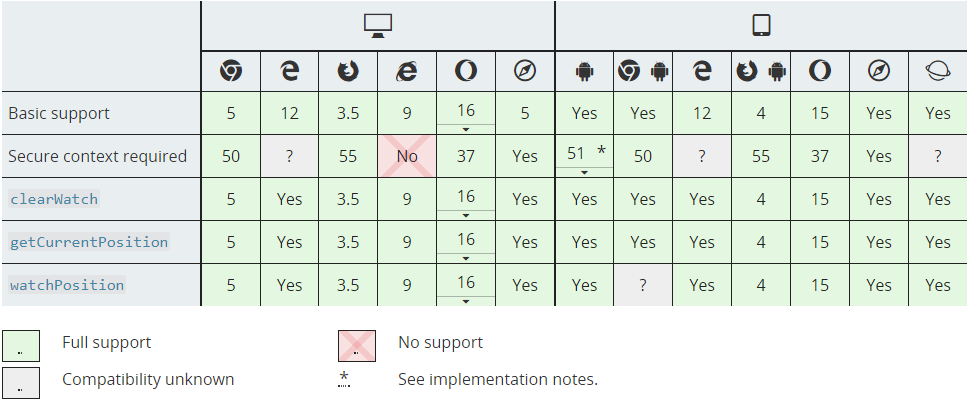
\includegraphics[width=1\linewidth]{compatibility}
	\caption{Desktop and mobile compatibility}
	\label{fig: Desktop and mobile compatibility}
\end{figure}
\newpage
\section{Conclusioni}
\newpage
\listoffigures
\newpage
\begin{thebibliography}{99}
	\bibitem{}
	 Connorshea, Chris David Mills, HeilKing, northvanhooser, erikadoyle, fscholz, Alhadis, teoli, FabioMagnoni (2018),
	 \emph{Features restricted to secure contexts, Mozilla Developer},
	\url{https://developer.mozilla.org/en-US/docs/Web/API/Geolocation}
	
	\bibitem{}
	heppy, Nisarg-Shah, tacsipacsi, chrisdavidmills, andysh, aneditor, smalllong, edent, divyanshu013, erikadoyle, VAggrippino, bsvensson, ewape, jpmedley, bjohnson, jsx, mugsydylan, Sebastianz, bizzybetz, shaneriley, atrama, nikifor, openjck, teoli, rebloor, Jeremie, jswisher, GARAAD, Zupper, jyz19880823, krishnachandra, markg, kohei.yoshino, kscarfone, SarahWalrus, BrandonLove, kmaglione, wlach, trevorh, ronj, ethertank, lmorchard, DavidWalsh, JohnKarahalis, mikerhodes, dflanagan, fcheslack, eberon, inma610, paul.irish, sebmozilla, dynamis, Steffen, stevep98, Dougt, Soupdragon, Chtitux, Bzbarsky
	\emph{Geolocation API, Mozilla Developer},
	\url{https://developer.mozilla.org/en-US/docs/Web/API/Geolocation_API}
	
	\bibitem{}
	W3C (2018), 
	\emph{Geolocation API Specification 2nd Edition},
	\url{https://www.w3.org/TR/geolocation-API/}
	
	\bibitem{}
	Ioannis Krontiris, Andreas Albers and Kai Rannenberg,
	\emph{W3C Geolocation API calls for
		Better User Privacy Protection}, 
	Chair of Mobile Business and Multilateral Security, Goethe University, Frankfurt, Germany
	
	\bibitem{}
	Doty, Nick, Mulligan, Deirdre K., Wilde, Erik (2010),
	\emph{Privacy Issues of the W3C Geolocation API}, UC Berkeley School of Information, \url{https://escholarship.org/uc/item/0rp834wf}
	
	\bibitem{}
	Ruadhán O'Donoghue (2013),
	\emph{HTML5 for the Mobile Web – a guide to the Geolocation API}, \url{https://mobiforge.com/design-development/html5-mobile-web-a-guide-geolocation-api}

	\bibitem{}
	OccupyTheWeb, WonderHowTo (2015),
	\emph{How to Find the Exact Location of Any IP Address}, \url{https://null-byte.wonderhowto.com/how-to/hack-like-pro-find-exact-location-any-ip-address-0161964/}
	
	\bibitem{}
	Kipkay(2017), 
	\emph{Trace Any IP Address}, \url{https://internet.gadgethacks.com/how-to/trace-any-ip-address-1916/}
	
	\bibitem{}
	Aurelio De Rosa (2014),
	\emph{An Introduction to the Geolocation API},
	\url{https://code.tutsplus.com/tutorials/an-introduction-to-the-geolocation-api--cms-20071}
	
	\bibitem{}
	Rafay Baloch, HTML5,
	\emph{HTML5 Modern Day Attack And Defense Vector},
	\url{http://www.xss-payloads.com/papers/HTML5AttackVectors.pdf}
\end{thebibliography}
\end{document}